
\documentclass{report}
\usepackage{blindtext}
\usepackage{enumerate}

%%%%%%%%%%%%%%%%%%%%%%%%%%%%%%%%%
% PACKAGE IMPORTS
%%%%%%%%%%%%%%%%%%%%%%%%%%%%%%%%%


\usepackage[tmargin=2cm,rmargin=1in,lmargin=1in,margin=0.85in,bmargin=2cm,footskip=.2in]{geometry}
\usepackage{amsmath,amsfonts,amsthm,amssymb,mathtools}
\usepackage[varbb]{newpxmath}
\usepackage{xfrac}
\usepackage[makeroom]{cancel}
\usepackage{mathtools}
\usepackage{bookmark}
\usepackage{enumitem}
\usepackage{hyperref,theoremref}
\hypersetup{
	pdftitle={Assignment},
	colorlinks=true, linkcolor=doc!90,
	bookmarksnumbered=true,
	bookmarksopen=true
}
\usepackage[most,many,breakable]{tcolorbox}
\usepackage{xcolor}
\usepackage{varwidth}
\usepackage{varwidth}
\usepackage{etoolbox}
%\usepackage{authblk}
\usepackage{nameref}
\usepackage{multicol,array}
\usepackage{tikz-cd}
\usepackage[ruled,vlined,linesnumbered]{algorithm2e}
\usepackage{comment} % enables the use of multi-line comments (\ifx \fi) 
\usepackage{import}
\usepackage{xifthen}
\usepackage{pdfpages}
\usepackage{transparent}

% Custom packages
\usepackage{bold-extra}
\usepackage{lmodern}
\usepackage{array}
\usepackage{pgfplots}
	\pgfplotsset{compat=1.18}
\usepackage[utf8]{inputenc}
\usepackage[T1]{fontenc}


\newcommand\mycommfont[1]{\footnotesize\ttfamily\textcolor{blue}{#1}}
\SetCommentSty{mycommfont}
\newcommand{\incfig}[1]{%
    \def\svgwidth{\columnwidth}
    \import{./figures/}{#1.pdf_tex}
}

\usepackage{tikzsymbols}
\renewcommand\qedsymbol{$\Laughey$}


%\usepackage{import}
%\usepackage{xifthen}
%\usepackage{pdfpages}
%\usepackage{transparent}


%%%%%%%%%%%%%%%%%%%%%%%%%%%%%%
% SELF MADE COLORS
%%%%%%%%%%%%%%%%%%%%%%%%%%%%%%



\definecolor{myg}{RGB}{56, 140, 70}
\definecolor{myb}{RGB}{45, 111, 177}
\definecolor{myr}{RGB}{199, 68, 64}
\definecolor{mytheorembg}{HTML}{F2F2F9}
\definecolor{mytheoremfr}{HTML}{00007B}
\definecolor{mylenmabg}{HTML}{FFFAF8}
\definecolor{mylenmafr}{HTML}{983b0f}
\definecolor{mypropbg}{HTML}{f2fbfc}
\definecolor{mypropfr}{HTML}{191971}
\definecolor{myexamplebg}{HTML}{F2FBF8}
\definecolor{myexamplefr}{HTML}{88D6D1}
\definecolor{myexampleti}{HTML}{2A7F7F}
\definecolor{mydefinitbg}{HTML}{E5E5FF}
\definecolor{mydefinitfr}{HTML}{3F3FA3}
\definecolor{notesgreen}{RGB}{0,162,0}
\definecolor{myp}{RGB}{197, 92, 212}
\definecolor{mygr}{HTML}{2C3338}
\definecolor{myred}{RGB}{127,0,0}
\definecolor{myyellow}{RGB}{169,121,69}
\definecolor{myexercisebg}{HTML}{F2FBF8}
\definecolor{myexercisefg}{HTML}{88D6D1}
% Custom Colors
\definecolor{sakura}{rgb}{0.99, 0.79, 0.73}
\definecolor{sakcomp}{rgb}{0.73, 0.93, 0.99}
\definecolor{iceblue}{rgb}{0.28, 0.79, 0.89}
\definecolor{deeppurple}{rgb}{0.70, 0.45, 1}

%%%%%%%%%%%%%%%%%%%%%%%%%%%%
% TCOLORBOX SETUPS
%%%%%%%%%%%%%%%%%%%%%%%%%%%%

\setlength{\parindent}{1cm}
%================================
% THEOREM BOX
%================================

\tcbuselibrary{theorems,skins,hooks}
\newtcbtheorem[number within=section]{Theorem}{Theorem}
{%
	enhanced,
	breakable,
	colback = mytheorembg,
	frame hidden,
	boxrule = 0sp,
	borderline west = {2pt}{0pt}{mytheoremfr},
	sharp corners,
	detach title,
	before upper = \tcbtitle\par\smallskip,
	coltitle = mytheoremfr,
	fonttitle = \bfseries\sffamily,
	description font = \mdseries,
	separator sign none,
	segmentation style={solid, mytheoremfr},
}
{th}

\tcbuselibrary{theorems,skins,hooks}
\newtcbtheorem[number within=chapter]{theorem}{Theorem}
{%
	enhanced,
	breakable,
	colback = mytheorembg,
	frame hidden,
	boxrule = 0sp,
	borderline west = {2pt}{0pt}{mytheoremfr},
	sharp corners,
	detach title,
	before upper = \tcbtitle\par\smallskip,
	coltitle = mytheoremfr,
	fonttitle = \bfseries\sffamily,
	description font = \mdseries,
	separator sign none,
	segmentation style={solid, mytheoremfr},
}
{th}


\tcbuselibrary{theorems,skins,hooks}
\newtcolorbox{Theoremcon}
{%
	enhanced
	,breakable
	,colback = mytheorembg
	,frame hidden
	,boxrule = 0sp
	,borderline west = {2pt}{0pt}{mytheoremfr}
	,sharp corners
	,description font = \mdseries
	,separator sign none
}

%================================
% Corollery
%================================
\tcbuselibrary{theorems,skins,hooks}
\newtcbtheorem[number within=section]{Corollary}{Corollary}
{%
	enhanced
	,breakable
	,colback = myp!10
	,frame hidden
	,boxrule = 0sp
	,borderline west = {2pt}{0pt}{myp!85!black}
	,sharp corners
	,detach title
	,before upper = \tcbtitle\par\smallskip
	,coltitle = myp!85!black
	,fonttitle = \bfseries\sffamily
	,description font = \mdseries
	,separator sign none
	,segmentation style={solid, myp!85!black}
}
{th}
\tcbuselibrary{theorems,skins,hooks}
\newtcbtheorem[number within=chapter]{corollary}{Corollary}
{%
	enhanced
	,breakable
	,colback = myp!10
	,frame hidden
	,boxrule = 0sp
	,borderline west = {2pt}{0pt}{myp!85!black}
	,sharp corners
	,detach title
	,before upper = \tcbtitle\par\smallskip
	,coltitle = myp!85!black
	,fonttitle = \bfseries\sffamily
	,description font = \mdseries
	,separator sign none
	,segmentation style={solid, myp!85!black}
}
{th}


%================================
% LENMA
%================================

\tcbuselibrary{theorems,skins,hooks}
\newtcbtheorem[number within=section]{Lenma}{Lenma}
{%
	enhanced,
	breakable,
	colback = mylenmabg,
	frame hidden,
	boxrule = 0sp,
	borderline west = {2pt}{0pt}{mylenmafr},
	sharp corners,
	detach title,
	before upper = \tcbtitle\par\smallskip,
	coltitle = mylenmafr,
	fonttitle = \bfseries\sffamily,
	description font = \mdseries,
	separator sign none,
	segmentation style={solid, mylenmafr},
}
{th}

\tcbuselibrary{theorems,skins,hooks}
\newtcbtheorem[number within=chapter]{lenma}{Lenma}
{%
	enhanced,
	breakable,
	colback = mylenmabg,
	frame hidden,
	boxrule = 0sp,
	borderline west = {2pt}{0pt}{mylenmafr},
	sharp corners,
	detach title,
	before upper = \tcbtitle\par\smallskip,
	coltitle = mylenmafr,
	fonttitle = \bfseries\sffamily,
	description font = \mdseries,
	separator sign none,
	segmentation style={solid, mylenmafr},
}
{th}


%================================
% PROPOSITION
%================================

\tcbuselibrary{theorems,skins,hooks}
\newtcbtheorem[number within=section]{Prop}{Proposition}
{%
	enhanced,
	breakable,
	colback = mypropbg,
	frame hidden,
	boxrule = 0sp,
	borderline west = {2pt}{0pt}{mypropfr},
	sharp corners,
	detach title,
	before upper = \tcbtitle\par\smallskip,
	coltitle = mypropfr,
	fonttitle = \bfseries\sffamily,
	description font = \mdseries,
	separator sign none,
	segmentation style={solid, mypropfr},
}
{th}

\tcbuselibrary{theorems,skins,hooks}
\newtcbtheorem[number within=chapter]{prop}{Proposition}
{%
	enhanced,
	breakable,
	colback = mypropbg,
	frame hidden,
	boxrule = 0sp,
	borderline west = {2pt}{0pt}{mypropfr},
	sharp corners,
	detach title,
	before upper = \tcbtitle\par\smallskip,
	coltitle = mypropfr,
	fonttitle = \bfseries\sffamily,
	description font = \mdseries,
	separator sign none,
	segmentation style={solid, mypropfr},
}
{th}


%================================
% CLAIM
%================================

\tcbuselibrary{theorems,skins,hooks}
\newtcbtheorem[number within=section]{claim}{Claim}
{%
	enhanced
	,breakable
	,colback = myg!10
	,frame hidden
	,boxrule = 0sp
	,borderline west = {2pt}{0pt}{myg}
	,sharp corners
	,detach title
	,before upper = \tcbtitle\par\smallskip
	,coltitle = myg!85!black
	,fonttitle = \bfseries\sffamily
	,description font = \mdseries
	,separator sign none
	,segmentation style={solid, myg!85!black}
}
{th}



%================================
% Exercise
%================================

\tcbuselibrary{theorems,skins,hooks}
\newtcbtheorem[number within=section]{Exercise}{Exercise}
{%
	enhanced,
	breakable,
	colback = myexercisebg,
	frame hidden,
	boxrule = 0sp,
	borderline west = {2pt}{0pt}{myexercisefg},
	sharp corners,
	detach title,
	before upper = \tcbtitle\par\smallskip,
	coltitle = myexercisefg,
	fonttitle = \bfseries\sffamily,
	description font = \mdseries,
	separator sign none,
	segmentation style={solid, myexercisefg},
}
{th}

\tcbuselibrary{theorems,skins,hooks}
\newtcbtheorem[number within=chapter]{exercise}{Exercise}
{%
	enhanced,
	breakable,
	colback = myexercisebg,
	frame hidden,
	boxrule = 0sp,
	borderline west = {2pt}{0pt}{myexercisefg},
	sharp corners,
	detach title,
	before upper = \tcbtitle\par\smallskip,
	coltitle = myexercisefg,
	fonttitle = \bfseries\sffamily,
	description font = \mdseries,
	separator sign none,
	segmentation style={solid, myexercisefg},
}
{th}

%================================
% EXAMPLE BOX
%================================

\newtcbtheorem[number within=section]{Example}{Example}
{%
	colback = myexamplebg
	,breakable
	,colframe = myexamplefr
	,coltitle = myexampleti
	,boxrule = 1pt
	,sharp corners
	,detach title
	,before upper=\tcbtitle\par\smallskip
	,fonttitle = \bfseries
	,description font = \mdseries
	,separator sign none
	,description delimiters parenthesis
}
{ex}

\newtcbtheorem[number within=chapter]{example}{Example}
{%
	colback = myexamplebg
	,breakable
	,colframe = myexamplefr
	,coltitle = myexampleti
	,boxrule = 1pt
	,sharp corners
	,detach title
	,before upper=\tcbtitle\par\smallskip
	,fonttitle = \bfseries
	,description font = \mdseries
	,separator sign none
	,description delimiters parenthesis
}
{ex}

%================================
% DEFINITION BOX
%================================

\newtcbtheorem[number within=section]{Definition}{Definition}{enhanced,
	before skip=2mm,after skip=2mm, colback=red!5,colframe=red!80!black,boxrule=0.5mm,
	attach boxed title to top left={xshift=1cm,yshift*=1mm-\tcboxedtitleheight}, varwidth boxed title*=-3cm,
	boxed title style={frame code={
					\path[fill=tcbcolback]
					([yshift=-1mm,xshift=-1mm]frame.north west)
					arc[start angle=0,end angle=180,radius=1mm]
					([yshift=-1mm,xshift=1mm]frame.north east)
					arc[start angle=180,end angle=0,radius=1mm];
					\path[left color=tcbcolback!60!black,right color=tcbcolback!60!black,
						middle color=tcbcolback!80!black]
					([xshift=-2mm]frame.north west) -- ([xshift=2mm]frame.north east)
					[rounded corners=1mm]-- ([xshift=1mm,yshift=-1mm]frame.north east)
					-- (frame.south east) -- (frame.south west)
					-- ([xshift=-1mm,yshift=-1mm]frame.north west)
					[sharp corners]-- cycle;
				},interior engine=empty,
		},
	fonttitle=\bfseries,
	title={#2},#1}{def}
\newtcbtheorem[number within=chapter]{definition}{Definition}{enhanced,
	before skip=2mm,after skip=2mm, colback=red!5,colframe=red!80!black,boxrule=0.5mm,
	attach boxed title to top left={xshift=1cm,yshift*=1mm-\tcboxedtitleheight}, varwidth boxed title*=-3cm,
	boxed title style={frame code={
					\path[fill=tcbcolback]
					([yshift=-1mm,xshift=-1mm]frame.north west)
					arc[start angle=0,end angle=180,radius=1mm]
					([yshift=-1mm,xshift=1mm]frame.north east)
					arc[start angle=180,end angle=0,radius=1mm];
					\path[left color=tcbcolback!60!black,right color=tcbcolback!60!black,
						middle color=tcbcolback!80!black]
					([xshift=-2mm]frame.north west) -- ([xshift=2mm]frame.north east)
					[rounded corners=1mm]-- ([xshift=1mm,yshift=-1mm]frame.north east)
					-- (frame.south east) -- (frame.south west)
					-- ([xshift=-1mm,yshift=-1mm]frame.north west)
					[sharp corners]-- cycle;
				},interior engine=empty,
		},
	fonttitle=\bfseries,
	title={#2},#1}{def}



%================================
% Solution BOX
%================================

\makeatletter
\newtcbtheorem{question}{Question}{enhanced,
	breakable,
	colback=white,
	colframe=myb!80!black,
	attach boxed title to top left={yshift*=-\tcboxedtitleheight},
	fonttitle=\bfseries,
	title={#2},
	boxed title size=title,
	boxed title style={%
			sharp corners,
			rounded corners=northwest,
			colback=tcbcolframe,
			boxrule=0pt,
		},
	underlay boxed title={%
			\path[fill=tcbcolframe] (title.south west)--(title.south east)
			to[out=0, in=180] ([xshift=5mm]title.east)--
			(title.center-|frame.east)
			[rounded corners=\kvtcb@arc] |-
			(frame.north) -| cycle;
		},
	#1
}{def}
\makeatother

%================================
% SOLUTION BOX
%================================

\makeatletter
\newtcolorbox{solution}{enhanced,
	breakable,
	colback=white,
	colframe=myg!80!black,
	attach boxed title to top left={yshift*=-\tcboxedtitleheight},
	title=Solution,
	boxed title size=title,
	boxed title style={%
			sharp corners,
			rounded corners=northwest,
			colback=tcbcolframe,
			boxrule=0pt,
		},
	underlay boxed title={%
			\path[fill=tcbcolframe] (title.south west)--(title.south east)
			to[out=0, in=180] ([xshift=5mm]title.east)--
			(title.center-|frame.east)
			[rounded corners=\kvtcb@arc] |-
			(frame.north) -| cycle;
		},
}
\makeatother

%================================
% Question BOX
%================================

\makeatletter
\newtcbtheorem{qstion}{Question}{enhanced,
	breakable,
	colback=white,
	colframe=mygr,
	attach boxed title to top left={yshift*=-\tcboxedtitleheight},
	fonttitle=\bfseries,
	title={#2},
	boxed title size=title,
	boxed title style={%
			sharp corners,
			rounded corners=northwest,
			colback=tcbcolframe,
			boxrule=0pt,
		},
	underlay boxed title={%
			\path[fill=tcbcolframe] (title.south west)--(title.south east)
			to[out=0, in=180] ([xshift=5mm]title.east)--
			(title.center-|frame.east)
			[rounded corners=\kvtcb@arc] |-
			(frame.north) -| cycle;
		},
	#1
}{def}
\makeatother

\newtcbtheorem[number within=chapter]{wconc}{Wrong Concept}{
	breakable,
	enhanced,
	colback=white,
	colframe=myr,
	arc=0pt,
	outer arc=0pt,
	fonttitle=\bfseries\sffamily\large,
	colbacktitle=myr,
	attach boxed title to top left={},
	boxed title style={
			enhanced,
			skin=enhancedfirst jigsaw,
			arc=3pt,
			bottom=0pt,
			interior style={fill=myr}
		},
	#1
}{def}



%================================
% NOTE BOX
%================================

\usetikzlibrary{arrows,calc,shadows.blur}
\tcbuselibrary{skins}
\newtcolorbox{note}[1][]{%
	enhanced jigsaw,
	colback=gray!20!white,%
	colframe=gray!80!black,
	size=small,
	boxrule=1pt,
	title=\textbf{Note:-},
	halign title=flush center,
	coltitle=black,
	breakable,
	drop shadow=black!50!white,
	attach boxed title to top left={xshift=1cm,yshift=-\tcboxedtitleheight/2,yshifttext=-\tcboxedtitleheight/2},
	minipage boxed title=1.5cm,
	boxed title style={%
			colback=white,
			size=fbox,
			boxrule=1pt,
			boxsep=2pt,
			underlay={%
					\coordinate (dotA) at ($(interior.west) + (-0.5pt,0)$);
					\coordinate (dotB) at ($(interior.east) + (0.5pt,0)$);
					\begin{scope}
						\clip (interior.north west) rectangle ([xshift=3ex]interior.east);
						\filldraw [white, blur shadow={shadow opacity=60, shadow yshift=-.75ex}, rounded corners=2pt] (interior.north west) rectangle (interior.south east);
					\end{scope}
					\begin{scope}[gray!80!black]
						\fill (dotA) circle (2pt);
						\fill (dotB) circle (2pt);
					\end{scope}
				},
		},
	#1,
}


%%%%%%%%%%%%%%%%%%%%%%%%%%%%%%
% SELF MADE COMMANDS
%%%%%%%%%%%%%%%%%%%%%%%%%%%%%%


\newcommand{\thm}[2]{\begin{Theorem}{#1}{}#2\end{Theorem}}
\newcommand{\cor}[2]{\begin{Corollary}{#1}{}#2\end{Corollary}}
\newcommand{\mlenma}[2]{\begin{Lenma}{#1}{}#2\end{Lenma}}
\newcommand{\mprop}[2]{\begin{Prop}{#1}{}#2\end{Prop}}
\newcommand{\clm}[3]{\begin{claim}{#1}{#2}#3\end{claim}}
\newcommand{\wc}[2]{\begin{wconc}{#1}{}\setlength{\parindent}{1cm}#2\end{wconc}}
\newcommand{\thmcon}[1]{\begin{Theoremcon}{#1}\end{Theoremcon}}
\newcommand{\ex}[2]{\begin{Example}{#1}{}#2\end{Example}}
\newcommand{\dfn}[2]{\begin{Definition}[colbacktitle=red!75!black]{#1}{}#2\end{Definition}}
\newcommand{\dfnc}[2]{\begin{definition}[colbacktitle=red!75!black]{#1}{}#2\end{definition}}
\newcommand{\qs}[2]{\begin{question}{#1}{}#2\end{question}}
\newcommand{\pf}[2]{\begin{myproof}[#1]#2\end{myproof}}
\newcommand{\nt}[1]{\begin{note}#1\end{note}}

\newcommand*\circled[1]{\tikz[baseline=(char.base)]{
		\node[shape=circle,draw,inner sep=1pt] (char) {#1};}}
\newcommand\getcurrentref[1]{%
	\ifnumequal{\value{#1}}{0}
	{??}
	{\the\value{#1}}%
}
\newcommand{\getCurrentSectionNumber}{\getcurrentref{section}}
\newenvironment{myproof}[1][\proofname]{%
	\proof[\bfseries #1: ]%
}{\endproof}

\newcommand{\mclm}[2]{\begin{myclaim}[#1]#2\end{myclaim}}
\newenvironment{myclaim}[1][\claimname]{\proof[\bfseries #1: ]}{}

\newcounter{mylabelcounter}

\makeatletter
\newcommand{\setword}[2]{%
	\phantomsection
	#1\def\@currentlabel{\unexpanded{#1}}\label{#2}%
}
\makeatother




\tikzset{
	symbol/.style={
			draw=none,
			every to/.append style={
					edge node={node [sloped, allow upside down, auto=false]{$#1$}}}
		}
}


% deliminators
\DeclarePairedDelimiter{\abs}{\lvert}{\rvert}
\DeclarePairedDelimiter{\norm}{\lVert}{\rVert}

\DeclarePairedDelimiter{\ceil}{\lceil}{\rceil}
\DeclarePairedDelimiter{\floor}{\lfloor}{\rfloor}
\DeclarePairedDelimiter{\round}{\lfloor}{\rceil}

\newsavebox\diffdbox
\newcommand{\slantedromand}{{\mathpalette\makesl{d}}}
\newcommand{\makesl}[2]{%
\begingroup
\sbox{\diffdbox}{$\mathsurround=0pt#1\mathrm{#2}$}%
\pdfsave
\pdfsetmatrix{1 0 0.2 1}%
\rlap{\usebox{\diffdbox}}%
\pdfrestore
\hskip\wd\diffdbox
\endgroup
}
\newcommand{\dd}[1][]{\ensuremath{\mathop{}\!\ifstrempty{#1}{%
\slantedromand\@ifnextchar^{\hspace{0.2ex}}{\hspace{0.1ex}}}%
{\slantedromand\hspace{0.2ex}^{#1}}}}
\ProvideDocumentCommand\dv{o m g}{%
  \ensuremath{%
    \IfValueTF{#3}{%
      \IfNoValueTF{#1}{%
        \frac{\dd #2}{\dd #3}%
      }{%
        \frac{\dd^{#1} #2}{\dd #3^{#1}}%
      }%
    }{%
      \IfNoValueTF{#1}{%
        \frac{\dd}{\dd #2}%
      }{%
        \frac{\dd^{#1}}{\dd #2^{#1}}%
      }%
    }%
  }%
}
\providecommand*{\pdv}[3][]{\frac{\partial^{#1}#2}{\partial#3^{#1}}}
%  - others
\DeclareMathOperator{\Lap}{\mathcal{L}}
\DeclareMathOperator{\Var}{Var} % varience
\DeclareMathOperator{\Cov}{Cov} % covarience
\DeclareMathOperator{\E}{E} % expected

% Since the amsthm package isn't loaded

% I prefer the slanted \leq
\let\oldleq\leq % save them in case they're every wanted
\let\oldgeq\geq
\renewcommand{\leq}{\leqslant}
\renewcommand{\geq}{\geqslant}

% % redefine matrix env to allow for alignment, use r as default
% \renewcommand*\env@matrix[1][r]{\hskip -\arraycolsep
%     \let\@ifnextchar\new@ifnextchar
%     \array{*\c@MaxMatrixCols #1}}


%\usepackage{framed}
%\usepackage{titletoc}
%\usepackage{etoolbox}
%\usepackage{lmodern}


%\patchcmd{\tableofcontents}{\contentsname}{\sffamily\contentsname}{}{}

%\renewenvironment{leftbar}
%{\def\FrameCommand{\hspace{6em}%
%		{\color{myyellow}\vrule width 2pt depth 6pt}\hspace{1em}}%
%	\MakeFramed{\parshape 1 0cm \dimexpr\textwidth-6em\relax\FrameRestore}\vskip2pt%
%}
%{\endMakeFramed}

%\titlecontents{chapter}
%[0em]{\vspace*{2\baselineskip}}
%{\parbox{4.5em}{%
%		\hfill\Huge\sffamily\bfseries\color{myred}\thecontentspage}%
%	\vspace*{-2.3\baselineskip}\leftbar\textsc{\small\chaptername~\thecontentslabel}\\\sffamily}
%{}{\endleftbar}
%\titlecontents{section}
%[8.4em]
%{\sffamily\contentslabel{3em}}{}{}
%{\hspace{0.5em}\nobreak\itshape\color{myred}\contentspage}
%\titlecontents{subsection}
%[8.4em]
%{\sffamily\contentslabel{3em}}{}{}  
%{\hspace{0.5em}\nobreak\itshape\color{myred}\contentspage}



%%%%%%%%%%%%%%%%%%%%%%%%%%%%%%%%%%%%%%%%%%%
% TABLE OF CONTENTS
%%%%%%%%%%%%%%%%%%%%%%%%%%%%%%%%%%%%%%%%%%%

\usepackage{tikz}
\definecolor{doc}{RGB}{0,60,110}
\usepackage{titletoc}
\contentsmargin{0cm}
\titlecontents{chapter}[3.7pc]
{\addvspace{30pt}%
	\begin{tikzpicture}[remember picture, overlay]%
		\draw[fill=doc!60,draw=doc!60] (-7,-.1) rectangle (-0.9,.5);%
		\pgftext[left,x=-3.5cm,y=0.2cm]{\color{white}\Large\sc\bfseries Chapter\ \thecontentslabel};%
	\end{tikzpicture}\color{doc!60}\large\sc\bfseries}%
{}
{}
{\;\titlerule\;\large\sc\bfseries Page \thecontentspage
	\begin{tikzpicture}[remember picture, overlay]
		\draw[fill=doc!60,draw=doc!60] (2pt,0) rectangle (4,0.1pt);
	\end{tikzpicture}}%
\titlecontents{section}[3.7pc]
{\addvspace{2pt}}
{\contentslabel[\thecontentslabel]{2pc}}
{}
{\hfill\small \thecontentspage}
[]
\titlecontents*{subsection}[3.7pc]
{\addvspace{-1pt}\small}
{}
{}
{\ --- \small\thecontentspage}
[ \textbullet\ ][]

\makeatletter
\renewcommand{\tableofcontents}{%
	\chapter*{%
	  \vspace*{-20\p@}%
	  \begin{tikzpicture}[remember picture, overlay]%
		  \pgftext[right,x=15cm,y=0.2cm]{\color{doc!60}\Huge\sc\bfseries \contentsname};%
		  \draw[fill=doc!60,draw=doc!60] (13,-.75) rectangle (20,1);%
		  \clip (13,-.75) rectangle (20,1);
		  \pgftext[right,x=15cm,y=0.2cm]{\color{white}\Huge\sc\bfseries \contentsname};%
	  \end{tikzpicture}}%
	\@starttoc{toc}}
\makeatother

%%%%%%%%%%%%%%%%%%%%%%%%%%%%%%%%%%%%%%%%%%%
% Personalized Commands and Such
%%%%%%%%%%%%%%%%%%%%%%%%%%%%%%%%%%%%%%%%%%%

%================================
% Are You Prepared Box
%================================

\newtcbtheorem[number within=section]{Prepared}{Are You Prepared?}{enhanced,
	before skip=2mm,after skip=2mm, colback=iceblue!5,colframe=iceblue!80!black,boxrule=0.5mm,
	attach boxed title to top left={xshift=1cm,yshift*=1mm-\tcboxedtitleheight}, varwidth boxed title*=-3cm,
	boxed title style={frame code={
					\path[fill=tcbcolback]
					([yshift=-1mm,xshift=-1mm]frame.north west)
					arc[start angle=0,end angle=180,radius=1mm]
					([yshift=-1mm,xshift=1mm]frame.north east)
					arc[start angle=180,end angle=0,radius=1mm];
					\path[left color=tcbcolback!60!black,right color=tcbcolback!60!black,
						middle color=tcbcolback!80!black]
					([xshift=-2mm]frame.north west) -- ([xshift=2mm]frame.north east)
					[rounded corners=1mm]-- ([xshift=1mm,yshift=-1mm]frame.north east)
					-- (frame.south east) -- (frame.south west)
					-- ([xshift=-1mm,yshift=-1mm]frame.north west)
					[sharp corners]-- cycle;
				},interior engine=empty,
		},
	fonttitle=\bfseries,
	title={#2},#1}{arp}
\newtcbtheorem[number within=chapter]{prepared}{Are You Prepared?}{enhanced,
	before skip=2mm,after skip=2mm, colback=iceblue!5,colframe=iceblue!80!black,boxrule=0.5mm,
	attach boxed title to top left={xshift=1cm,yshift*=1mm-\tcboxedtitleheight}, varwidth boxed title*=-3cm,
	boxed title style={frame code={
					\path[fill=tcbcolback]
					([yshift=-1mm,xshift=-1mm]frame.north west)
					arc[start angle=0,end angle=180,radius=1mm]
					([yshift=-1mm,xshift=1mm]frame.north east)
					arc[start angle=180,end angle=0,radius=1mm];
					\path[left color=tcbcolback!60!black,right color=tcbcolback!60!black,
						middle color=tcbcolback!80!black]
					([xshift=-2mm]frame.north west) -- ([xshift=2mm]frame.north east)
					[rounded corners=1mm]-- ([xshift=1mm,yshift=-1mm]frame.north east)
					-- (frame.south east) -- (frame.south west)
					-- ([xshift=-1mm,yshift=-1mm]frame.north west)
					[sharp corners]-- cycle;
				},interior engine=empty,
		},
	fonttitle=\bfseries,
	title={#2},#1}{arp}

\newcommand{\arp}[2]{\begin{Prepared}[colbacktitle=iceblue!75!black]{#1}{}#2\end{Prepared}}

%================================
% Refactoring Commands
%================================


%================================
% New Characters
%================================
%From M275 "Topology" at SJSU
\newcommand{\id}{\mathrm{id}}
\newcommand{\taking}[1]{\xrightarrow{#1}}
\newcommand{\inv}{^{-1}}

%From M170 "Introduction to Graph Theory" at SJSU
\DeclareMathOperator{\diam}{diam}
\DeclareMathOperator{\ord}{ord}
\newcommand{\defeq}{\overset{\mathrm{def}}{=}}

%From the USAMO .tex files
\newcommand{\ts}{\textsuperscript}
\newcommand{\dg}{^\circ}
\newcommand{\ii}{\item}

% % From Math 55 and Math 145 at Harvard
% \newenvironment{subproof}[1][Proof]{%
% \begin{proof}[#1] \renewcommand{\qedsymbol}{$\blacksquare$}}%
% {\end{proof}}

\newcommand\shortlorem{pp|pp}
\newcommand{\liff}{\leftrightarrow}
\newcommand{\lthen}{\rightarrow}
\newcommand{\opname}{\operatorname}
\newcommand{\surjto}{\twoheadrightarrow}
\newcommand{\injto}{\hookrightarrow}
\newcommand{\On}{\mathrm{On}} % ordinals
\DeclareMathOperator{\img}{im} % Image
\DeclareMathOperator{\Img}{Im} % Image
\DeclareMathOperator{\coker}{coker} % Cokernel
\DeclareMathOperator{\Coker}{Coker} % Cokernel
\DeclareMathOperator{\Ker}{Ker} % Kernel
\DeclareMathOperator{\rank}{rank}
\DeclareMathOperator{\Spec}{Spec} % spectrum
\DeclareMathOperator{\Tr}{Tr} % trace
\DeclareMathOperator{\pr}{pr} % projection
\DeclareMathOperator{\ext}{ext} % extension
\DeclareMathOperator{\pred}{pred} % predecessor
\DeclareMathOperator{\dom}{dom} % domain
\DeclareMathOperator{\ran}{ran} % range
\DeclareMathOperator{\Hom}{Hom} % homomorphism
\DeclareMathOperator{\Mor}{Mor} % morphisms
\DeclareMathOperator{\End}{End} % endomorphism

\newcommand{\eps}{\epsilon}
\newcommand{\veps}{\varepsilon}
\newcommand{\ol}{\overline}
\newcommand{\ul}{\underline}
\newcommand{\wt}{\widetilde}
\newcommand{\wh}{\widehat}
\newcommand{\vocab}[1]{\textbf{\color{blue} #1}}
\providecommand{\half}{\frac{1}{2}}
\newcommand{\dang}{\measuredangle} %% Directed angle
\newcommand{\ray}[1]{\overrightarrow{#1}}
\newcommand{\seg}[1]{\overline{#1}}
\newcommand{\arc}[1]{\wideparen{#1}}
\DeclareMathOperator{\cis}{cis}
\DeclareMathOperator*{\lcm}{lcm}
\DeclareMathOperator*{\argmin}{arg min}
\DeclareMathOperator*{\argmax}{arg max}
\newcommand{\cycsum}{\sum_{\mathrm{cyc}}}
\newcommand{\symsum}{\sum_{\mathrm{sym}}}
\newcommand{\cycprod}{\prod_{\mathrm{cyc}}}
\newcommand{\symprod}{\prod_{\mathrm{sym}}}
\newcommand{\Qed}{\begin{flushright}\qed\end{flushright}}
\newcommand{\parinn}{\setlength{\parindent}{1cm}}
\newcommand{\parinf}{\setlength{\parindent}{0cm}}
% \newcommand{\norm}{\|\cdot\|}
\newcommand{\inorm}{\norm_{\infty}}
\newcommand{\opensets}{\{V_{\alpha}\}_{\alpha\in I}}
\newcommand{\oset}{V_{\alpha}}
\newcommand{\opset}[1]{V_{\alpha_{#1}}}
\newcommand{\lub}{\text{lub}}
\newcommand{\del}[2]{\frac{\partial #1}{\partial #2}}
\newcommand{\Del}[3]{\frac{\partial^{#1} #2}{\partial^{#1} #3}}
\newcommand{\deld}[2]{\dfrac{\partial #1}{\partial #2}}
\newcommand{\Deld}[3]{\dfrac{\partial^{#1} #2}{\partial^{#1} #3}}
\newcommand{\lm}{\lambda}
\newcommand{\uin}{\mathbin{\rotatebox[origin=c]{90}{$\in$}}}
\newcommand{\usubset}{\mathbin{\rotatebox[origin=c]{90}{$\subset$}}}
\newcommand{\lt}{\left}
\newcommand{\rt}{\right}
\newcommand{\bs}[1]{\boldsymbol{#1}}
\newcommand{\exs}{\exists}
\newcommand{\st}{\strut}
\newcommand{\dps}[1]{\displaystyle{#1}}

\newcommand{\sol}{\setlength{\parindent}{0cm}\textbf{\textit{Solution:}}\setlength{\parindent}{1cm} }
\newcommand{\solve}[1]{\setlength{\parindent}{0cm}\textbf{\textit{Solution: }}\setlength{\parindent}{1cm}#1 \Qed}
% Things Lie
\newcommand{\kb}{\mathfrak b}
\newcommand{\kg}{\mathfrak g}
\newcommand{\kh}{\mathfrak h}
\newcommand{\kn}{\mathfrak n}
\newcommand{\ku}{\mathfrak u}
\newcommand{\kz}{\mathfrak z}
\DeclareMathOperator{\Ext}{Ext} % Ext functor
\DeclareMathOperator{\Tor}{Tor} % Tor functor
\newcommand{\gl}{\opname{\mathfrak{gl}}} % frak gl group
\renewcommand{\sl}{\opname{\mathfrak{sl}}} % frak sl group chktex 6

% More script letters etc.
\newcommand{\SA}{\mathcal A}
\newcommand{\SB}{\mathcal B}
\newcommand{\SC}{\mathcal C}
\newcommand{\SF}{\mathcal F}
\newcommand{\SG}{\mathcal G}
\newcommand{\SH}{\mathcal H}
\newcommand{\OO}{\mathcal O}

\newcommand{\SCA}{\mathscr A}
\newcommand{\SCB}{\mathscr B}
\newcommand{\SCC}{\mathscr C}
\newcommand{\SCD}{\mathscr D}
\newcommand{\SCE}{\mathscr E}
\newcommand{\SCF}{\mathscr F}
\newcommand{\SCG}{\mathscr G}
\newcommand{\SCH}{\mathscr H}

% Mathfrak primes
\newcommand{\km}{\mathfrak m}
\newcommand{\kp}{\mathfrak p}
\newcommand{\kq}{\mathfrak q}

% number sets
\newcommand{\RR}[1][]{\ensuremath{\ifstrempty{#1}{\mathbb{R}}{\mathbb{R}^{#1}}}}
\newcommand{\NN}[1][]{\ensuremath{\ifstrempty{#1}{\mathbb{N}}{\mathbb{N}^{#1}}}}
\newcommand{\ZZ}[1][]{\ensuremath{\ifstrempty{#1}{\mathbb{Z}}{\mathbb{Z}^{#1}}}}
\newcommand{\QQ}[1][]{\ensuremath{\ifstrempty{#1}{\mathbb{Q}}{\mathbb{Q}^{#1}}}}
\newcommand{\CC}[1][]{\ensuremath{\ifstrempty{#1}{\mathbb{C}}{\mathbb{C}^{#1}}}}
\newcommand{\PP}[1][]{\ensuremath{\ifstrempty{#1}{\mathbb{P}}{\mathbb{P}^{#1}}}}
\newcommand{\HH}[1][]{\ensuremath{\ifstrempty{#1}{\mathbb{H}}{\mathbb{H}^{#1}}}}
\newcommand{\FF}[1][]{\ensuremath{\ifstrempty{#1}{\mathbb{F}}{\mathbb{F}^{#1}}}}
% expected value
\newcommand{\EE}{\ensuremath{\mathbb{E}}}
\newcommand{\charin}{\text{ char }}
\DeclareMathOperator{\sign}{sign}
\DeclareMathOperator{\Aut}{Aut}
\DeclareMathOperator{\Inn}{Inn}
\DeclareMathOperator{\Syl}{Syl}
\DeclareMathOperator{\Gal}{Gal}
\DeclareMathOperator{\GL}{GL} % General linear group
\DeclareMathOperator{\SL}{SL} % Special linear group

%---------------------------------------
% BlackBoard Math Fonts :-
%---------------------------------------

%Captital Letters
\newcommand{\bbA}{\mathbb{A}}	\newcommand{\bbB}{\mathbb{B}}
\newcommand{\bbC}{\mathbb{C}}	\newcommand{\bbD}{\mathbb{D}}
\newcommand{\bbE}{\mathbb{E}}	\newcommand{\bbF}{\mathbb{F}}
\newcommand{\bbG}{\mathbb{G}}	\newcommand{\bbH}{\mathbb{H}}
\newcommand{\bbI}{\mathbb{I}}	\newcommand{\bbJ}{\mathbb{J}}
\newcommand{\bbK}{\mathbb{K}}	\newcommand{\bbL}{\mathbb{L}}
\newcommand{\bbM}{\mathbb{M}}	\newcommand{\bbN}{\mathbb{N}}
\newcommand{\bbO}{\mathbb{O}}	\newcommand{\bbP}{\mathbb{P}}
\newcommand{\bbQ}{\mathbb{Q}}	\newcommand{\bbR}{\mathbb{R}}
\newcommand{\bbS}{\mathbb{S}}	\newcommand{\bbT}{\mathbb{T}}
\newcommand{\bbU}{\mathbb{U}}	\newcommand{\bbV}{\mathbb{V}}
\newcommand{\bbW}{\mathbb{W}}	\newcommand{\bbX}{\mathbb{X}}
\newcommand{\bbY}{\mathbb{Y}}	\newcommand{\bbZ}{\mathbb{Z}}

%---------------------------------------
% MathCal Fonts :-
%---------------------------------------

%Captital Letters
\newcommand{\mcA}{\mathcal{A}}	\newcommand{\mcB}{\mathcal{B}}
\newcommand{\mcC}{\mathcal{C}}	\newcommand{\mcD}{\mathcal{D}}
\newcommand{\mcE}{\mathcal{E}}	\newcommand{\mcF}{\mathcal{F}}
\newcommand{\mcG}{\mathcal{G}}	\newcommand{\mcH}{\mathcal{H}}
\newcommand{\mcI}{\mathcal{I}}	\newcommand{\mcJ}{\mathcal{J}}
\newcommand{\mcK}{\mathcal{K}}	\newcommand{\mcL}{\mathcal{L}}
\newcommand{\mcM}{\mathcal{M}}	\newcommand{\mcN}{\mathcal{N}}
\newcommand{\mcO}{\mathcal{O}}	\newcommand{\mcP}{\mathcal{P}}
\newcommand{\mcQ}{\mathcal{Q}}	\newcommand{\mcR}{\mathcal{R}}
\newcommand{\mcS}{\mathcal{S}}	\newcommand{\mcT}{\mathcal{T}}
\newcommand{\mcU}{\mathcal{U}}	\newcommand{\mcV}{\mathcal{V}}
\newcommand{\mcW}{\mathcal{W}}	\newcommand{\mcX}{\mathcal{X}}
\newcommand{\mcY}{\mathcal{Y}}	\newcommand{\mcZ}{\mathcal{Z}}


%---------------------------------------
% Bold Math Fonts :-
%---------------------------------------

%Captital Letters
\newcommand{\bmA}{\boldsymbol{A}}	\newcommand{\bmB}{\boldsymbol{B}}
\newcommand{\bmC}{\boldsymbol{C}}	\newcommand{\bmD}{\boldsymbol{D}}
\newcommand{\bmE}{\boldsymbol{E}}	\newcommand{\bmF}{\boldsymbol{F}}
\newcommand{\bmG}{\boldsymbol{G}}	\newcommand{\bmH}{\boldsymbol{H}}
\newcommand{\bmI}{\boldsymbol{I}}	\newcommand{\bmJ}{\boldsymbol{J}}
\newcommand{\bmK}{\boldsymbol{K}}	\newcommand{\bmL}{\boldsymbol{L}}
\newcommand{\bmM}{\boldsymbol{M}}	\newcommand{\bmN}{\boldsymbol{N}}
\newcommand{\bmO}{\boldsymbol{O}}	\newcommand{\bmP}{\boldsymbol{P}}
\newcommand{\bmQ}{\boldsymbol{Q}}	\newcommand{\bmR}{\boldsymbol{R}}
\newcommand{\bmS}{\boldsymbol{S}}	\newcommand{\bmT}{\boldsymbol{T}}
\newcommand{\bmU}{\boldsymbol{U}}	\newcommand{\bmV}{\boldsymbol{V}}
\newcommand{\bmW}{\boldsymbol{W}}	\newcommand{\bmX}{\boldsymbol{X}}
\newcommand{\bmY}{\boldsymbol{Y}}	\newcommand{\bmZ}{\boldsymbol{Z}}
%Small Letters
\newcommand{\bma}{\boldsymbol{a}}	\newcommand{\bmb}{\boldsymbol{b}}
\newcommand{\bmc}{\boldsymbol{c}}	\newcommand{\bmd}{\boldsymbol{d}}
\newcommand{\bme}{\boldsymbol{e}}	\newcommand{\bmf}{\boldsymbol{f}}
\newcommand{\bmg}{\boldsymbol{g}}	\newcommand{\bmh}{\boldsymbol{h}}
\newcommand{\bmi}{\boldsymbol{i}}	\newcommand{\bmj}{\boldsymbol{j}}
\newcommand{\bmk}{\boldsymbol{k}}	\newcommand{\bml}{\boldsymbol{l}}
\newcommand{\bmm}{\boldsymbol{m}}	\newcommand{\bmn}{\boldsymbol{n}}
\newcommand{\bmo}{\boldsymbol{o}}	\newcommand{\bmp}{\boldsymbol{p}}
\newcommand{\bmq}{\boldsymbol{q}}	\newcommand{\bmr}{\boldsymbol{r}}
\newcommand{\bms}{\boldsymbol{s}}	\newcommand{\bmt}{\boldsymbol{t}}
\newcommand{\bmu}{\boldsymbol{u}}	\newcommand{\bmv}{\boldsymbol{v}}
\newcommand{\bmw}{\boldsymbol{w}}	\newcommand{\bmx}{\boldsymbol{x}}
\newcommand{\bmy}{\boldsymbol{y}}	\newcommand{\bmz}{\boldsymbol{z}}

%---------------------------------------
% Scr Math Fonts :-
%---------------------------------------

\newcommand{\sA}{{\mathscr{A}}}   \newcommand{\sB}{{\mathscr{B}}}
\newcommand{\sC}{{\mathscr{C}}}   \newcommand{\sD}{{\mathscr{D}}}
\newcommand{\sE}{{\mathscr{E}}}   \newcommand{\sF}{{\mathscr{F}}}
\newcommand{\sG}{{\mathscr{G}}}   \newcommand{\sH}{{\mathscr{H}}}
\newcommand{\sI}{{\mathscr{I}}}   \newcommand{\sJ}{{\mathscr{J}}}
\newcommand{\sK}{{\mathscr{K}}}   \newcommand{\sL}{{\mathscr{L}}}
\newcommand{\sM}{{\mathscr{M}}}   \newcommand{\sN}{{\mathscr{N}}}
\newcommand{\sO}{{\mathscr{O}}}   \newcommand{\sP}{{\mathscr{P}}}
\newcommand{\sQ}{{\mathscr{Q}}}   \newcommand{\sR}{{\mathscr{R}}}
\newcommand{\sS}{{\mathscr{S}}}   \newcommand{\sT}{{\mathscr{T}}}
\newcommand{\sU}{{\mathscr{U}}}   \newcommand{\sV}{{\mathscr{V}}}
\newcommand{\sW}{{\mathscr{W}}}   \newcommand{\sX}{{\mathscr{X}}}
\newcommand{\sY}{{\mathscr{Y}}}   \newcommand{\sZ}{{\mathscr{Z}}}


%---------------------------------------
% Math Fraktur Font
%---------------------------------------

%Captital Letters
\newcommand{\mfA}{\mathfrak{A}}	\newcommand{\mfB}{\mathfrak{B}}
\newcommand{\mfC}{\mathfrak{C}}	\newcommand{\mfD}{\mathfrak{D}}
\newcommand{\mfE}{\mathfrak{E}}	\newcommand{\mfF}{\mathfrak{F}}
\newcommand{\mfG}{\mathfrak{G}}	\newcommand{\mfH}{\mathfrak{H}}
\newcommand{\mfI}{\mathfrak{I}}	\newcommand{\mfJ}{\mathfrak{J}}
\newcommand{\mfK}{\mathfrak{K}}	\newcommand{\mfL}{\mathfrak{L}}
\newcommand{\mfM}{\mathfrak{M}}	\newcommand{\mfN}{\mathfrak{N}}
\newcommand{\mfO}{\mathfrak{O}}	\newcommand{\mfP}{\mathfrak{P}}
\newcommand{\mfQ}{\mathfrak{Q}}	\newcommand{\mfR}{\mathfrak{R}}
\newcommand{\mfS}{\mathfrak{S}}	\newcommand{\mfT}{\mathfrak{T}}
\newcommand{\mfU}{\mathfrak{U}}	\newcommand{\mfV}{\mathfrak{V}}
\newcommand{\mfW}{\mathfrak{W}}	\newcommand{\mfX}{\mathfrak{X}}
\newcommand{\mfY}{\mathfrak{Y}}	\newcommand{\mfZ}{\mathfrak{Z}}
%Small Letters
\newcommand{\mfa}{\mathfrak{a}}	\newcommand{\mfb}{\mathfrak{b}}
\newcommand{\mfc}{\mathfrak{c}}	\newcommand{\mfd}{\mathfrak{d}}
\newcommand{\mfe}{\mathfrak{e}}	\newcommand{\mff}{\mathfrak{f}}
\newcommand{\mfg}{\mathfrak{g}}	\newcommand{\mfh}{\mathfrak{h}}
\newcommand{\mfi}{\mathfrak{i}}	\newcommand{\mfj}{\mathfrak{j}}
\newcommand{\mfk}{\mathfrak{k}}	\newcommand{\mfl}{\mathfrak{l}}
\newcommand{\mfm}{\mathfrak{m}}	\newcommand{\mfn}{\mathfrak{n}}
\newcommand{\mfo}{\mathfrak{o}}	\newcommand{\mfp}{\mathfrak{p}}
\newcommand{\mfq}{\mathfrak{q}}	\newcommand{\mfr}{\mathfrak{r}}
\newcommand{\mfs}{\mathfrak{s}}	\newcommand{\mft}{\mathfrak{t}}
\newcommand{\mfu}{\mathfrak{u}}	\newcommand{\mfv}{\mathfrak{v}}
\newcommand{\mfw}{\mathfrak{w}}	\newcommand{\mfx}{\mathfrak{x}}
\newcommand{\mfy}{\mathfrak{y}}	\newcommand{\mfz}{\mathfrak{z}}
\graphicspath{ {./images/APBIO} }

\title{\Huge{AP Biology}\\ Notes}
\author{Me. I am Him.}
\date{11/28/2022}

\begin{document}

\maketitle
\newpage
\pdfbookmark[section]{\contentsname}{toc}
\tableofcontents
\pagebreak

\thispagestyle{empty}
\newpage
\listoffigures
\clearpage
\pagenumbering{arabic}


\chapter{Chemistry of Life}
\section{Scientific Method}
\section{Feedback}
\nt{Positive and Negative feedback. Need to know.}
\section{Macromolecules}


\newpage
\chapter{Cell Structure and Function}\label{ch:cell-structure-and-function}
\nt{\textbf{All} cells have the following;
    \begin{enumerate}
        \item Surrounding Membrane
        \item Chromosomes
        \item Cytosol
        \item Ribosomes.
    \end{enumerate}}
\dfn{Prokaryotic Cells}{They are defined as being, having, or including:
    \begin{enumerate}
        \item Non-membrane-bound organelles
        \item Nucleoid
    \end{enumerate}
    \nt{Prokaryotes include \textit{Bacteria} and \textit{Archaea}. They both differ genetically.}}
\dfn{Eukaryotic Cells}{They are defined as being, having, or including:
    \begin{enumerate}
        \item Membrane-bound organelles, including a nucleus.
        \item Multicellular potential.
    \end{enumerate}
    \nt{There is a limit on how big a cell can get. This is defined by the square-cube law. As surface area squares, the volume gets cubed.}}
\thm{Cellular Evolution}{Current Evidence indicates that eukaryotes evolved from prokaryotes between 1 and 1.5 billion years ago.
\nt{There are two current theories on howthis happened:
    \begin{enumerate}
        \item Folding Theory: In short, we believe that parts of the cell membrane folded in on itself, pinched off, and became specialized cells.
        \item Endosymbiotic Theory: The \textit{mitochondria} and \textit{chloroplasts} were once prokaryotic and somehow and for some reason became incorporated into another cell.
    \end{enumerate}}}

\section{Organelles}\label{sec:organelles}
\dfn{Organelle}{Insert Def here.}
\dfn{Nucleus}{Manager of cell functions. It also contains DNA and the nucleolus.}
\dfn{Nuclear Membrane}{A double membrane, each made up of two layers, making four total. It is selectively porous.}
\dfn{Nucleolus}{A darker spot in the nucleus where RNA and ribosomes are made.}
\dfn{Ribosome}{Produces proteins; made in the nucleolus}
\dfn{Endomembrane System}{Made up of all internal membranes in a cell; a continuous system. Vesicles bud off from and attach to membrane systems; transport shuttles.}
\dfn{Endoplasmic Reticulum}{Two Types;
    \begin{enumerate}
        \item [-] Smooth: No ribosomes.
        \item [-] Rough: Has ribosomes.
    \end{enumerate}}
\dfn{Vesicles}{Transporters.}
\dfn{Golgi Body/Apparatus}{Packages proteins; leaves on the trans side.}
\dfn{Lysosome}{Breaks down things; contains digestive enzymes.}
\dfn{Vacuole}{Store things, such as water.}
\dfn{Plastids}{Double Membrane.
\nt{\textit{Plastid}, a double membrane $\neq$ \textit{Plasmid}, prokaryotic DNA}}


\chapter{DNA}\label{ch:dna}
\section{DNA and Replication}

\dfn{DNA}{Hereditary information that is found inall cells of the body.}
\nt{DNA Contains the information to make proteins and directs the development of biochemical, atomical, physiological, and --to some extent-- behavioral traits.}

\subsection{Frederick Griffith}

\begin{center}
	Frederick Griffith worked with two strains of a bacterium, a pathogen "S" strain and a harmless "R" strain. He investigated what happened when they were each injected into a mouse.
	\begin{tabular}{rl}
		& $\bullet$ Living 'S' cells = dead mouse \\
		& $\bullet$ Living 'R' cells = alive mouse \\
		& $\bullet$ Heat killed 'S' cells = alive mouse \\
		& $\bullet$ Living 'R' cells + heat killed 'S' cells = dead mouse. \\
	\end{tabular}
	\nt{Note how the mouse is alive with heat killed 'S' cells but dead when those cells are added to 'R' cells. In conclusion, the heat killed 'S' cells are able to infect and take over the living 'R' cells and subsequently kill the mouse.}
\end{center}

\subsection{Structure}
\dfn{Double Helix}{Specifically, DNA is two anti-parallel sugar-phosphate backbones, with the ntriogenous bases paired in the molecules interior.}
\nt{All nitrogen bases have a specific partener. For example, Thymine (T) only goes with Adenine (A), and Guanine (G) only goes with Cytosine (C).}

\subsection{Packaging and Organization}
\dfn{Chromatin}{DNA and all associated proteins.}
\dfn{Heterochromatin}{Highly Compacted DNA}
\dfn{Euchromatin}{DNA that is able to be transcribed.}
\nt{If there is no DNA, or the DNA cannot be transcribed, no proteins will be made}
\qs{How is DNA packaged?}{
	\begin{enumerate}
		\item The DNA is wrapped around a \textbf{histone} twice.
	\item Eight histones are then gathered, creating a line. A sort-of beads-on-a-string. These are called \textbf{Nucleosomes}.
	\item These nucleosomes eventually clump up, creating many loop shapes, called \textbf{looped domains}.
	\item These looped domains eventually organize into \textbf{Metaphase chromosomes}.
	\end{enumerate}
\dfn{Histone}{A group of basic proteins found in chromatin. Their tails can be modified.}
\dfn{Nucleosome}{A structural unit of a eukaryotic chromosome, consisting of a determined length of DNA coiled around a core of histones.}
\dfn{Looped Domain}{A basic structural unit of eukaryotic chromatin associated with DNA replication, gene expression, and higher order packaging.}
\dfn{Metaphase Chromosome}{Simply a chromosome in the stage of \textit{metaphase} of the cell cycle.}}

\newpage
\section{DNA Replication}
\dfn{DNA Replication}{The process by which DNA is replicated. It follows a \textit{semi-conservative model}.}
\dfn{Semi-conservative model}{A process where there is one original and one new strand.}
\nt{Copying DNA is easy due to the hydrogen bonds holding the bases together, but also hard thanks to DNA being antiparallel.}
\ex{DNA Replication}{
	\begin{enumerate}
		\item Helicase untwists the DNA and seperates the strands. This is only done in sections. It starts at specific DNA sequences.
		\item Topoisomerase relieves the pressure from the bubble. The bubble forms thanks to helicase working in sections.
		\item Primase then deposits primers from the middle of the buble towards the 5` end.
		\item DNA polymerase III (DP3) adds DNA nucleotides to the 3` end of the primer. The hydrogen bond then forms between the new strand and old strand.
		\item DNA polymerase I (DP1) starts to remove the primer and replaces it with DNA nucleotides. This occurs from 3` to 5`
	\end{enumerate}
	\nt{If the template strand starts from the 3` to 5` end, the new strand will start from the 5` to 3`.}}

\dfn{Leading Strand}{The strand who leads from the half-way-point in the bubble.}
\dfn{Lagging Strand}{The strand who are made before the half-way-point and eventually catch up to the leading strand.
\nt{Individual parts to the lagging strand are called okizaki fragments. They are placed randomly.}}
\dfn{Primase}{Synthesizes RNA primers, using parenta DNA as a template.}
\dfn{Topoisomerase}{Breaks, swivels, and rejoins the parenta DNA ahead of the replication fork, relieving the strain caused by unwinding.}
\dfn{Helicase}{Unwinds and seperates the parental DNA strands.}
\dfn{Single-Strand Binding}{satblize the unwound parental strands.}



\newpage
\section{Genetic Engineering}
\ex{How to Genetic Engineer}{
	\begin{enumerate}
		\item Take a gene and put it into a bacteria
		\item The bacteria will then express the gene and produce the protein.
		\item Extract the protein.
	\end{enumerate}}
\dfn{Transgeneic Organism}{An organism containing DNA from two differing sources.}
\dfn{Recombinant DNA}{A mixed genome derived from two differing sources.}
\dfn{Nucleic Acid Hybridization}{The property where one strand of DNA is complimentary, and therefore will connect to another strand.
	\nt{
		\begin{enumerate}
			\item If you heat up DNA, the strands separate.
			\item If you add a strand that is complimentary and is radioactive, you can find that section. This is used in the \textbf{chain termination method}
		\end{enumerate}}}


\subsection{Cloning}
\dfn{Polymerase Chain Reaction (PCR)}{A process by which sections of a DNA sample is amplified. The process is done in a thermocycler.}
\begin{figure}[h]
	\centering
	\caption{Polymerase Chain Reaction}
	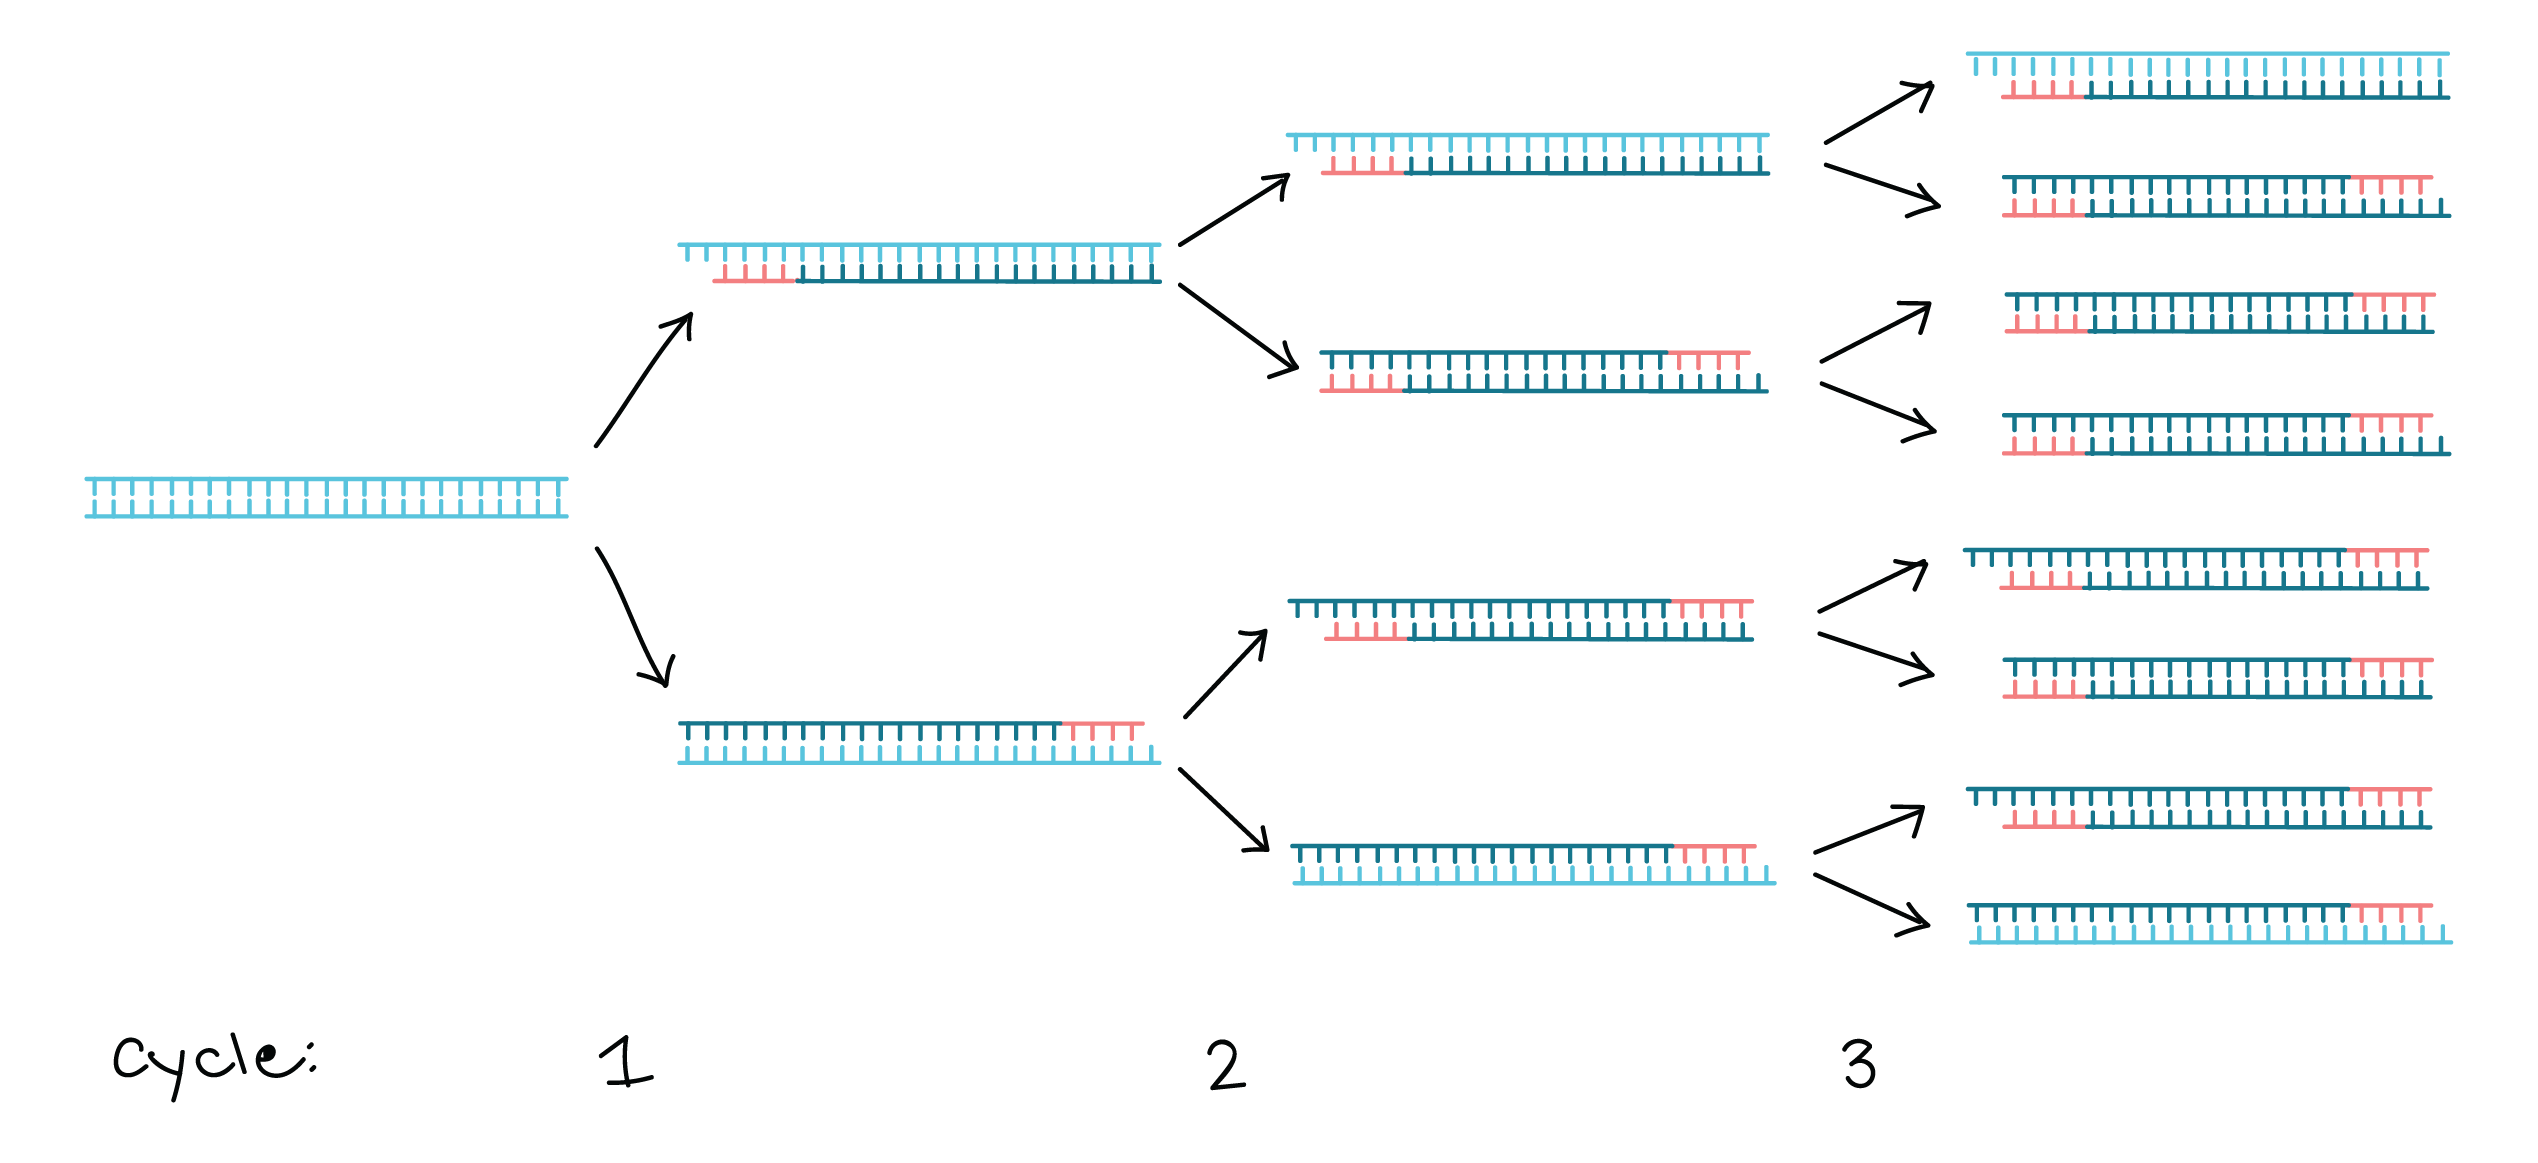
\includegraphics[scale=0.6]{Chapter 13 - PCR.png} 
	\label{PCR}
\end{figure}
\dfn{Restriction Enzyme}{Cleaves DNA sequences as sequence-specific sites, producing DNA fragments with a known sequence at each end.}

\subsection{Sequencing the Genone}
\dfn{Chain Termination Method}{The process by which we add complimentary DNA nucleotides to a known section of DNA. We use a \textbf{thermocycler} to automate this process.
	\nt{Whether the thermocycler chooses a marked nucleotide or not is random. However, when it chooses a marked nucleotide, the process stops.}}
\nt{To analyze the DNA, we use \textit{Gel Electrophoresis}. This sorts them by size and charge.}
\dfn{Restriction Fragment Length Polymorphisms (RFLP's)}{A variation in the length of restriction fragments produced by a given restriction enzyme in a sample of DNA. 
	\nt{Different people have different fragment lengths.}}
	\dfn{Dideoxyidenucleotide}{}


\newpage
\section{Gel Electrophoresis}
\dfn{Gel Electrophorisis}{The process by which you measure and sort strands of DNA, proteins, or other molecules.} 
\qs{How does it work?}{
	$\bullet$ A gel-like filter with many small holes in it sorts the DNA strands. \\
	$\bullet$ First, we place some DNA samples into one end of the filter. \\
	$\bullet$ Second, we run electricity through it, creating a positive and negative end which pushes the DNA strands through the filter. This is where the 'electrophoresis' comes from. \\
	$\bullet$ We can tell which are longer and which are shorter by looking at how far each strand traveled. Shorter strands will travel farther over time. \\
	$\bullet$ We can then stain the sorted groups of DNA, allowing the naked eye to see them. We don't see individual strands, though, we see the groups of them.
	\nt{Fragments are sorted by \textbf{size} and \textbf{charge}. Smaller molecules go farther.}}
\begin{figure}[h]
	\centering
	\caption{Gel Electrophoresis}
	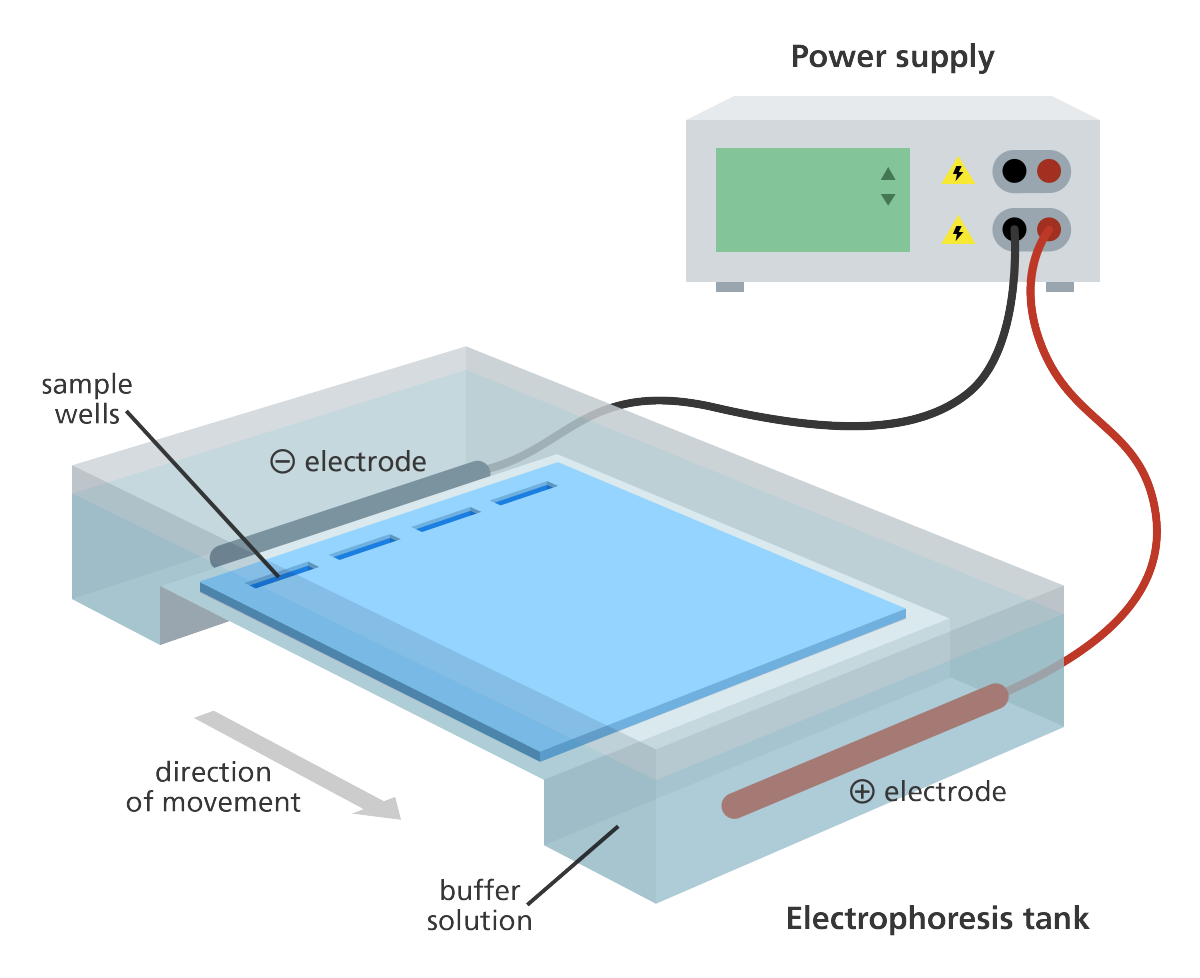
\includegraphics[scale=0.3]{Chapter 13 - Gel Electrophoresis.png}
	\label{Gel Electrophoresis}
\end{figure}

\pagebreak
\section{Editing Genes}
\dfn{CRISPR-Cas9}{Clustered Regularly Interspaced Short Palindromic Repeats. This protein has the ability to llcate, cut, and repair or disable a specific \textit{gene}.
	\nt{It was first discovered in bacteriophages as protection against viruses.}
	\nt{There are two parts:
		\begin{enumerate}
			\item Cas9 Protein: Nuclease enzyme that cuts double stranded DNA wherever it is brought.
			\item Guide RNA: Complimentary piece of RNA that binds to a target gene.
		\end{enumerate}}
\nt{If you know the sequence of the gene, you can create the guide RNA.}}
\begin{figure}[h]
	\centering
	\caption{Cas9 RNA Targetting}
	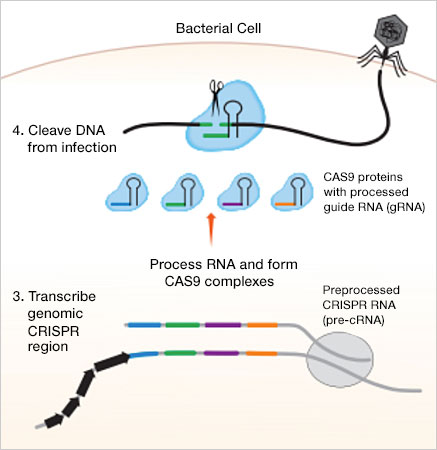
\includegraphics[scale=0.6]{Chapter 13 - Cas9 RNA.jpg} 
	\label{Cas9}
\end{figure}


\newpage
\section{Gene Expression}

\nt{Protein Synthesis requires two processes:
	DNA $\rightarrow$ RNA $\rightarrow$ Protein}
\dfn{Transcription}{Makes RNA.}
\dfn{Translation}{Makes Proteins.}
\nt{\textit{Transcription} takes place in the nucleus whereas \textit{Translation} takes place at ribosomes in the cytosol. Proteins are modified in the \textit{golgi body}.}

\subsection{The Genetic Code}
\dfn{Codon}{A set of 3 nitrogen bases in DNA that make an amino acid.}
\nt{Only one side of the DNA strand will be used as a template.}
\nt{AUG is the \textbf{ONLY} start codon. This is a must know.}
\nt{There are three stop codons. Memorize them. \textbf{UAA}, \textbf{UGA}, and \textbf{UAG}.}

\subsection{Transcription: Making RNA}
\nt{There are several different types of RNA, all with different shapes and functions. They are all made in the nucleus, but different RNA functions are made in different places. \textbf{Uracil} replaces \textbf{Thymine}.}
\dfn{Gene Unit}{The portion of DNA involved in transcription.}
\dfn{RNA Polymerase}{Like DNA polymerase, RNA polymerase makes RNA.}
\dfn{Promoter}{The part of DNA where RNA polymerase builds. Their purpose is to line up RNA polymerase's active site with the first base to be transcribed.
	\nt{It is 'upstream' from the start of the gene.}}
\dfn{Transcription factor}{HELLLLLLLLPPPPPPPPPPPPPPPPP}
\nt{Unlike how DNA can be copied off other DNA, RNA can \textbf{ONLY} be transcribed from RNA.}

\ex{Three Steps to Transcription:}{
\begin{enumerate}
	\item Initiation
	\item Elongation
	\item Termination
\end{enumerate}}
\dfn{Initiation}{Here, the transcription factors bind to the DNA, RNA polymerase binds to the right spot, and the RNA polymerase begins to unwind the DNA.}
\dfn{Elongation}{Here, RNA polymerase moves along the DNA, untwisting 10 to 20 bases at a time. The complimentary bases are added, and the DNA zips back up behind it. This happens at a rate of 60 nucleotides a second in eukaryotes.}
\dfn{Termination}{In \textit{prokaryotes}, it ends at the terminator. However, in \textit{eukaryotes}, it breaks off after a specific sequence.}

\newpage
\section{RNA Processing}
"""GO BACK TO THE FIRST SLIDES AND RECOPY THE SLIDES.
\nt{All RNA's are virtually the same, but \textit{mRNA} has the instructions to put the amino acids together in the correct order.}
\nt{Pre-\textit{mRNA} must be modified before it's sent to the cytoplasm.}


\subsection{Alteration of mRNA Ends}
\nt{The 5' end gets a Mg Cap. This helps it get out of the nucleus, protects it from degredation, and helps it bind to a ribosome.}
\nt{The 3' end gets a Poly-A tail. The longer the tail, the longer it lasts. It also acilitates the export of \textit{mRNA} from the nucleus and protects it from degredation.}
\dfn{Untranslated Regions}{The region between the mG cap and the coding sequence and between the stop codon and the poly-A tail.}

\subsection{RNA Splicing}
\dfn{RNA Splicing}{The process by which spliceosomes remove introns and push together extrons to create the final sequence.}
\dfn{Spliceosomes}{A conglomerate of various proteins and several small nuclear ribonucleoproteins(\textit{snRNP}s), or \textit{snurps} that recognize the splice sites.}
\dfn{Introns}{A non-coding sequence. They get spliced out and removed.}
\dfn{Extrons}{A coding sequence.They get spliced together after the introns are removed.}
\nt{Must remove introns, they are called spliceosomes. Think of RNA as a movie. Must remove deleted scenes (introns), push together the rest. The final directors cut is made up of the pre-roll (5' cap), the movie itself (extrons), and the credits (3' cap or Poly-A tail).}
\nt{Introns are important for one main reason. They lead to \textit{alternative RNA splicing.}}
\dfn{Alternative RNA Splicing}{The process by which different areas lead to different results from RNA splicing. This works thanks to some areas splicing out some exons.
	\nt{This is how we get hundreds of thousands of proteins from only 21,000 genes.}}

\subsection{Translation}\label{subsec:translation}
\dfn{Translation}{The process to convert the RNA code into a protein.
	\nt{It requires three different types of RNA:
	\begin{enumerate}
		\item mRNA
		\item tRNA
		\item rRNA
	\end{enumerate}}
	It also has three stages:
	\begin{enumerate}
		\item Initiation
		\item Elongation
		\item Termination
	\end{enumerate}}

\dfn{tRNA}{A single molecule consisting of a single RNA strand that is only about 80 nucleotides long.
\nt{It caries an animo acid on the 3` end. Loop two also contains a anti-codon, whcih means that it is complimentary to the codon it's using.}}
\dfn{Wobble}{The relaxing of base pairing on the third base of a(n) (anti)codon. In short, it explains why the third base in a codon can sometimes change without changing the overall protein.}

\subsection{Ribosomes}
\dfn{Ribosome}{Made up of two ribosomal units (large and small) are made up of proteins and \textit{rRNA}
	\nt{A ribosome has three binding sites for tRNA. These are in order:
	\begin{enumerate}
		\item A site: holds the tRNA that carries the next amino acid to be added to the chain.
		\item P site: holds the tRNA that carries the growing polypeptide chain.
		\item E site: is the exit site, where discharged tRNAs leave the ribosome.
	\end{enumerate}}}
\dfn{Initiation}{
	\begin{enumerate}
		\item Small ribosomal subunits binds to \textit{mRNA} (at the start of the codon AUG)
		\item tRNA (carrying methonine) binds to \textit{mRNA} in the P site.
		\item Large ribosomal subunit comes in and arranges itself to the tRNA in the P site.
	\end{enumerate}}
\dfn{Elongation}{
	\begin{enumerate}
		\item Second \textit{tRNA} entes the A-site; codon binds to the anti-codon.
		\item The amino acid on the \textit{tRNA} in the P site 'jumps back' and is bonded to the amino acid on the \textit{tRNA} in the A site.
		\item Translocation - the \textit{tRNA} in the P-site gets moved to the E-site where it gets kicked out while the \textit{tRNA} in the A-site gets moved to the P-site.
		\item Ribosomes move along \textit{mRNA} from 5` to 3`
		\item Repeat.
	\end{enumerate}}
\dfn{Release Factor}{When the ribosome encounters a stop codon, a release factor enters and binds a water molecule to the ribosome. This causes the polypeptide chain to break off from the strand and the ribosome releases.}


\subsection{Point Mutations}
\nt{There are two types of point mutation:
\begin{enumerate}
	\item Base-pair substitutions
	\item Base-pair insertions or deletions.
\end{enumerate}}

\dfn{Substitutions}{The replacement of one nucleotide and its partner with another pair of nucleotides.}
\dfn{Missense Mutation}{A mutation where it still codes for an amin acid, but it may not nessecarily be the correct one.}
\dfn{Nonsense Mutation}{A mutation where an amino acid codon is changed into a stop codon. This leads to a nonfunctional protein.}
\dfn{Insertions and Deletions}{The addition or removal of a nucleotide pair in a gene. This usually leads to massive issues in the reading and translation of the RNA. This is also called a frameshift mutation.}
\dfn{Mutagen}{Physical or chemical agents that can cause mutations. Examples include smoking, radioactivity, and more.}

\dfn{Lac Operon}{When would enzymes \textit{NOT} be made? -> 
\begin{enumerate}
	\item [-] When Lactose is NOT present.
	\item [-] When Glucose IS present.
\end{enumerate}}

\nt{Allolactose is another way to say lactose.}
\nt{The \textit{Lac} Operon and \textit{Trp} Operon are different in that the Lac prosessor (inhibitor) is made active, whereas the Trp processor (inhibitor) is made inactive.}
\dfn{Repressible Operon}{
	\begin{enumerate}
		\item [-] Usually Functions in anabolic pathways.
		\item [-] Synthesizing end products
		\item [-] When end product is present cell allocates to other uses.
		\item [-] Trp Operon.
		\item [-] Genes are active.
		\item [-] Regulatory protein (inhibitor) is made in the inactive form.
		\item [-] The things being made activates the regulatory protein when there is enough of that thing.
	\end{enumerate}}

\dfn{Inducible Operon}{
	\begin{enumerate}
		\item [-] Usually functions in catabolic pathways, digesting nutrients to simpler proteins.
		\item [-] Produce enzymes only when nutrient is available.
		\item [-] Cell avoids making proteins that have nothing to do.
		\item [-] Lac Operon.
		\item [-] Genes are inactive.
		\item [-] Regulatory Protein (inhibitor) is made in active form.
		\item [-] The thing being broken down inactivates the regulatory protein when that thing is around
	\end{enumerate}}

\nt{This \textit{ONLY} in Prokaryotes. Control in Eukaryotes is completely different thanks to their DNA being different.}

\ex{Control in Eukaryotes}{
	\begin{enumerate}
		\item DNA gets transcribed into pre-mRNA
		\item pre-mRNA gets spliced to the proper mRNA
		\item mRNA gets translated into proteins.
		\item The proteins then do their thing.
	\end{enumerate}
	We control this by stopping translation and transcription. It's hard to explain, but think of it as a main water line to your home.
	We stop the main line, then go throughout the house draining the individual sections by turning on the sink.}

\newpage
\section{Regulating DNA Structure}

\dfn{Histone Acetylation}{
	\begin{enumerate}
		\item [-] Acetylated histones seperate from each other; DNA is looser.
		\item [-] Why? Positive Charges are neutralized; no charge to attract.
		\item [-] Allows for transcription
	\end{enumerate}
}
\dfn{Methylation}{
	\begin{enumerate}
		\item [-] Adding methyl groups to DNA to prevent transcription.
		\item [-] Methyl groups are also added to histone proteins.
	\end{enumerate}
}
\dfn{Epigenetic Heriditation}{yo
}

\nt{Regulating Transcription Initiation:
	\begin{enumerate}
		\item [-] Preventing or allowing RNA polymerase
	\end{enumerate}
}
\dfn{Transciription Factor:}{
The things that control RNA polymerase in DNA interaction. RNA polymerase needs transcription factors in order to bind to DNA.
\nt{Two Types:
	\begin{enumerate}
		\item General: Needed for the transcription of \textit{ALL} protein genes.
		\item Specific: Needed to transcribe a specific gene. They bind to enhancer regions which are specific for a gene. Some may be activators, others are seperators.
		\item [In Short] You need both factors for RNA polyerase to attach. First the specific ones attach to the gene then the general factors attach to the specific ones.
		\item [Overview:] An activator (type of specific factor) binds to an enhancer (control element), and then DNA bends. A specific facor binds to the activator, which then has a general factor on top of that. RNA polymerase can now attach to the general factor.
	\end{enumerate}}}

\nt{Huge note: Repressors take the space that the activators take. They regulate the speed by stopping a factor from attaching, thus preventing RNA polymerase from attaching.}

\subsection{mRNA Degredation}
\nt{mRNA doesn't last forever. When it's gone, no more translation into a protein.
\begin{enumerate}
	\item Small segments of RNA that leads to the break down of mRNA.
	\item miRNA and siRNA (DON'T NEED TO KNOW THE DIFFERENCE. JUST THEIR NAMES)
	\item Both miRNA and siRNA are originally long pieces of \textit{double stranded} RNA.
	\item Double stranded RNA is then chopped up by a protein called \textit{Dicer} into the miRNA and siRNA.
Think of gum on a zipper. They prevent translation.
They attach to the untranslated regions. Untranslated regions are the areas between the spliced extrons and the m-G cap and the extrons and the poly-A tail.
miRNA \textit{desroyers}, well, destroy, the mRNA.
\end{enumerate}}

\dfn{Proteasomes}{Complex of proteins that break down proteins. A protein, called \textit{ubiquitin} marks the protein, and a proteasome comes in and breaks it down.}

\subsection{Monitoring Gene Expression}
\begin{enumerate}
	\item Nucleic Acid Hybridization
	\begin{itemize}
		\item Detects where a gene is being usedor expressed.
		\item Uses a nucleic acid probe (something with a fluorecent tag.)
		\item Looks for and attaches to the corresponding gene. (compliment)
	\end{itemize}
\end{enumerate}
\nt{Muscle and Brain cells have the same DNA, however, only the muscle cells make actin. This is because the gene [for actin] is only active in the mRNA in muscle cells.}
\dfn{PT-PCR}{
	\nt{PCR is used on DNA, RT-PCR is used on RNA.}
	\begin{enumerate}
		\item Reverse transcriptase-polymerase chain reacton.
		\item Compares the amount of a specific mRNA that is used.
		\item Uses reverse transcriptase
		\begin{itemize}
			\item Makes DNA from RNA. (The reverse of transcription)
		\end{itemize}
		\item Basically, you make a whole bunch of DNA from a piece of mRNA.
		\item The DNA that is made is called cDNA (Complimentary DNA)
		\item The Covid Test... 
	\end{enumerate}
}
\ex{
	\begin{enumerate}
		\item [First] Make the cDNA
		\item [Second] See how much cDNA is made
		\begin{itemize}
			\item The more cDNA that is ade, the more mRNA there was at the start
		\end{itemize}
		\item What does this tell you?
		\begin{itemize}
			\item It tells you how much a particular gene is being expressed in a specific type of cell.
		\end{itemize}
	\end{enumerate}
}

\nt{More on cDNA:
\begin{enumerate}
	\item cDNA is also what is needed to get a prokaryote to express a human gene.
	\item Why?
	Because \textit{prokaryotes} cannot splice.
\end{enumerate}
}

\subsection{Studying Groups of Genes}\label{subsec:studying-groups-of-genes}
\begin{itemize}
	\item DNA Micro-array Assays
	\begin{itemize}
		\item You get a chip (a micro-array)
		\item In a perfect world, the chip has every gene on It
		\item Bt you only have single strand DNA versions of each gene.
		\item mRNA's from cells you are studying are revere transcribed.
		\begin{itemize}
			\item This makes cDNA\@.
		\end{itemize}
		\item Make sure to use a fluorescent label to make those cDNA's.
		\item If you are studying 2 cells at the same time, each cell can have a different fluorescent colour.
		\item Add the cDNA to the chips
		\item Check the colours.
	\end{itemize}
\end{itemize}

\chapter{4: Cellular Communication}\label{ch:Cellular Comm.}

Cells must talk	to each other. They do this via signals or messengers, these are called ligands. Ligands is a general term for any signaling molecule.
Molecules made by some cells have an affect on others. For example, neurotransmitters communicate from one neuron to the next nerve cell or even muscle cell.
Cells in the immune system will either communicate with each other to help fight off an infection or cause an infected or cancerous cell to kill itself.
\qs{Whats the point?}{}
Recieving cells have proteins embedded in their membranes. These are called receptor proteins.

\section{Reception}\label{sec:reception}
\nt{The binding between signal molecule (ligand) and receptor is highly specific.}
\dfn{Conformational Change}{The process by which a protein changes shape via something attaching to said protein.}
\nt{There are two main types of membrane receptors.
\begin{enumerate}
	\item G-protein-coupled receptor
	\begin{itemize}
		\item Works with a G-protein (protein that turns on and off enzymes)
	\end{itemize}
	\item Ligand-gated ion chanel
	\begin{itemize}
		\item Open when ligand binds
	\end{itemize}
\end{enumerate}}
\ex{How G-protein-coupled receptor's work.}{
\begin{enumerate}
	\item Ligand (signal) attaches to GPCR protein (receptor) in the cellular membrane
	\item G protein (bound to the GPCR) becomes activated and moves to the inactive enzyme
	\item The previously inactive enzyme is now activated and produces the specific protein (cellular response).
\end{enumerate}}
\nt{Ligand Gated Ion Channels use channel proteins and are thus passive transport. They only use high $\rightarrow$ low gradients.}
\nt{\textbf{Intracellular Receptors}
\begin{itemize}
	\item Most ligands are large and water-soluble and must bind to membrane proteins.
	\item Other ligands are hydrophobic and enter the cell (such as steroids)
	\begin{itemize}
		\item They bind to intracellular receptors
	\end{itemize}
	\item They \textit{usually} are hormones.
	\item They \textit{usually} activate genes.
\end{itemize}}

\dfn{Transduction}{Transduction of a signal is a multistep pathway (signal transduction pathway.)
\nt{
\begin{itemize}
	\item Advantages:
	\begin{itemize}
		\item Can amplify a signal.
		\item Provide more opportunities for coordination and regulation
	\end{itemize}
	\item The signal is passed by proteins changing shape (usually due to phosphorylation
	\begin{itemize}
		\item Phosporylation = adding a P$_{i}$ (from ATP)
	\end{itemize}
\end{itemize}
}}
\nt{In this process;
\begin{itemize}
	\item A series of protein kinases add a phosphate to the next one in line, activating it
	\item Phosphatase enzymes then remove the phosphates (called protein phosphatases)
	\item Or in other words, 1 activates 2 which activates 3 which activates 4 until the response is made.
	\item Kinase's are called such because they \textit{phosphorylate} other molecules, not because they become phosphorylated.
\end{itemize}}

%insert photo from gyazo

\dfn{Second Messengers}{Small, nonprotein, water-soluble molecules or ions that activate proteins inside of a cell.
\begin{itemize}
	\item Most common second messengers are cAMP and Ca$^{2+}$
	\item These are the things that start the cascade
\end{itemize}}

\nt{Response:
\begin{enumerate}
    \item Activate/Deactivate an enzyme in the cytoplasm
    \item Turn on/off genes in the nucleus
\end{enumerate}}

\qs{Why so many steps?}{
\begin{enumerate}
	\item Amplification.
	\item Specificity.
	\begin{itemize}
		\item A cell will only respond if it has the right receptor.
		\item A ligand MAY be able to bind to two different receptors made by two different cells.
		\item There, however, you would get two different responses.
	\end{itemize}
\end{enumerate}
}
\nt{When the ligand leaves the receptor, the pathway stops. The signal response is terminated somewhat quickly.}

\nt{Feedbacks;
\begin{enumerate}
	\item Positive Feedback
	\begin{itemize}
		\item When the reaction enhances the original stimulus
		\item Amplification
		\item An end
	\end{itemize}
	\item Negative Feedback
	\begin{itemize}
		\item When the reaction counters the original stimulus
		\item Keep things in a narrow range.
	\end{itemize}
\end{enumerate}}

\section{The Cell Cycle}

\dfn{Phases:}{Interphase:G1, S, G2 | Mitosis.
Interphase:
\begin{enumerate}
	\item G1:
	\begin{itemize}
		\item Growth and normal cell functions
	\end{itemize}
	\item S
	\begin{itemize}
		\item DNA Replication
	\end{itemize}
	\item G2
	\begin{itemize}
		\item Preperation for Mitosis
	\end{itemize}
\end{enumerate}
Phases of Mitosis:
\begin{enumerate}
	\item Prophase
	\item Prometaphase (Do not need to know. College Board does not accept it as an answer right now.)
	\item Metaphase
	\item Anaphase
	\item Telophase and Cytokinesis
\end{enumerate}
}














\newpage
\begin{figure}
	\centering
	\Huge{Thanks for reading}
	
\includegraphics[scale=0.2]{dabloon}
	\label{fig:dabloonia}
\end{figure}

\end{document}
